\input ../SlidePreamble
\input ../preamble

\begin{document}

{\Huge

  \centerline{\bf TTIC 31230, Fundamentals of Deep Learning}
  \bigskip
  \centerline{David McAllester, Winter 2019}


\vfill
\centerline{\bf AlphaZero}
\vfill
\vfill

\slide{AlphaGo Fan (October 2015)}

AlphaGo Defeats Fan Hui, European Go Champion.

\vfill
\centerline{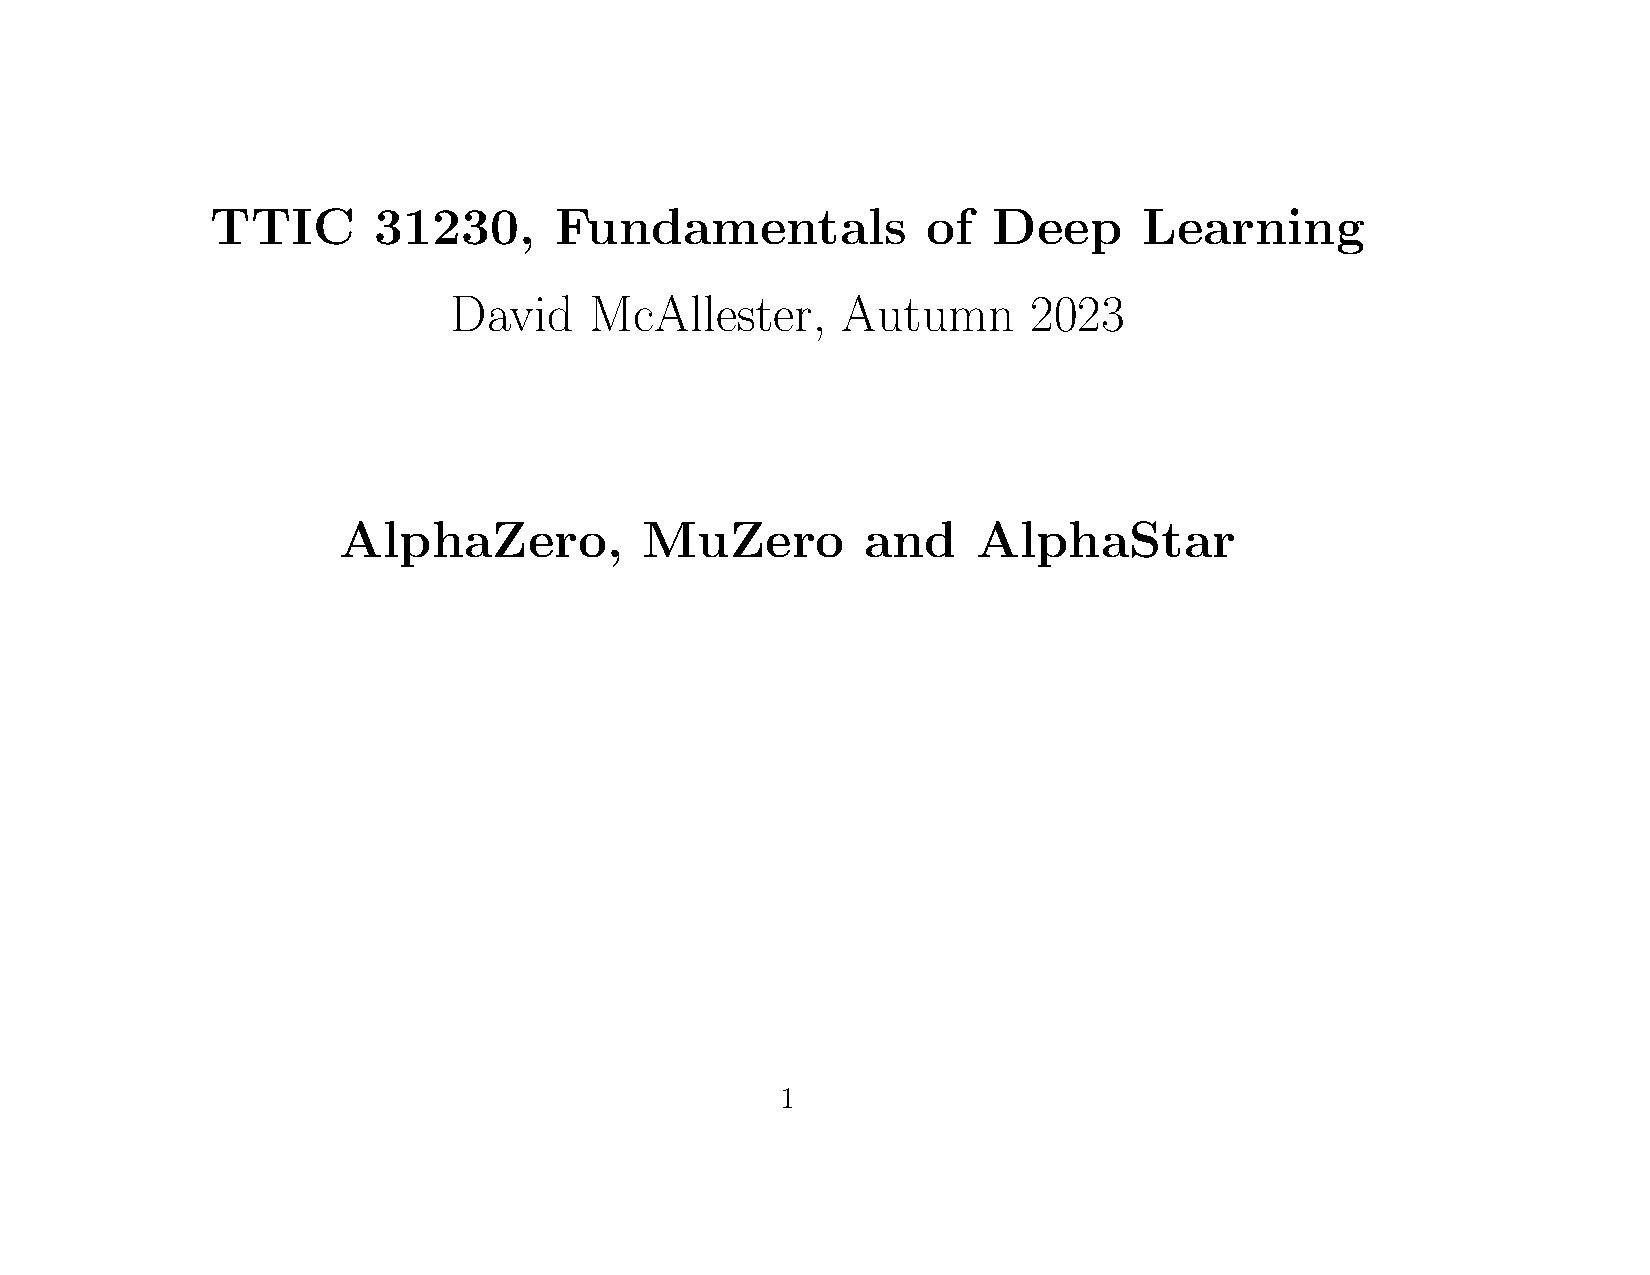
\includegraphics[width=4in]{../images/alphago}}

\slide{AlphaGo Lee (March 2016)}

\vfill
\centerline{\includegraphics[width=8in]{../images/alphagolee}}

\slide{AlphaGo Zero vs. Alphago Lee (April 2017)}

{\bf AlphaGo Lee:}

\begin{itemize}
\item Trained on both human games and self play.
  
\item Trained for Months.

\item Run on many machines with 48 TPUs for Lee Sedol match.
\end{itemize}

{\bf AlphaGo Zero:}
\begin{itemize}
\item Trained on self play only.
  
\item Trained for 3 days.

\item Run on one machine with 4 TPUs.

\item Defeated AlphaGo Lee under match conditions 100 to 0.
\end{itemize}

\slide{AlphaZero Defeats Stockfish in Chess (December 2017)}

AlphaGo Zero was a fundamental algorithmic advance for general RL.

\vfill
The general RL algorithm of AlphaZero is essentially the same as that of AlphaGo Zero.

\slide{}

\centerline{\bf Some Background}

\vfill

\slidetwo{Monte-Carlo Tree Search (MCTS)}
{Brugmann (1993)}

To estimate the value of a position (who is ahead and by how much)
run a cheap stochastic policy to generate a sequence of moves (a rollout) and see who wins.

\vfill
Select the move with the best rollout value.

\slidetwo{(One Armed) Bandit Problems}
{Robbins (1952)}

Consider a set of choices (different slot machines).

Each choice gets a stochastic reward.

\vfill
We can select a choice and get a reward as often as we like.

\vfill
We would like to determine which choice is best and also to get reward as quickly as possible.

\slidetwo{The Upper Confidence Bound (UCB) Algorithm}
{Lai and Robbins (1985)}

For each choice (bandit) $a$ construct a confidence interval for its average reward.

\vfill
$$\mu = \hat{\mu} \pm 2\sigma/\sqrt{n}$$

\vfill
$$\mu(a) \leq \hat{\mu}(a) + U(N(a))$$

\vfill
Always select

$$\argmax_a \hat{\mu}(a) + U(N(a))$$

\slidetwo{The Upper Confidence Tree (UCT) Algorithm}
{Kocsis and Szepesvari (2006), Gelly and Silver (2007)}

The UCT algorithm grows a tree by running ``simulations''.

\vfill
Each simulation descends into the tree to a leaf node, expands that leaf, and returns a value.

\vfill
In the UTC algorithm each move choice at each position is treated as a bandit problem.

\vfill
We select the child (bandit) with the the lowest upper bound as computed from revious simulations selecting that child.


\slidetwo{Bootstrapping from Game Tree Search}
{Vaness, Silver, Blair and Uther, NeurIPS 2009}

In bootstrapped tree search we do a tree search to compute a min-max value $V_{\mathrm{mm}}(s)$
using tree search with a static evaluator $V_\Phi(s)$.  We then try to fit the static value to the min-max value.

\vfill
$$\Delta \Phi = - \eta \nabla_\Phi \left(V_\Phi(s) - V_{\mathrm{mm}}(s)\right)^2$$

\vfill
This is similar to minimizing a Bellman error between $V_\Phi(s)$ and a rollout estimate of the value of $s$ but where the rollout
estimate is replaced by a min-max tree search estimate.

\slide{}

\centerline{\bf The AlphaZero Algorithm}
\bigskip
\centerline{\bf Silver et al. (2017)}

\vfill

\slide{The AlphaZero Algorithm}

The AlphaZero algorithm is an RL learning method for the case where state transitions are determined by actions.

\vfill
In principle, the AlphaZero algorithm could be applied to the problem of direct optimization of the BLEU score in machine translation.

\slide{Tree Search}

To select an action, first construct a search tree over possible action sequences to evaluate options.

\vfill
As in UTC, the tree is grown by running simulations.  Each simulation descends into the tree from the root selecting an action at each state until a new leaf is created.

\vfill
In an adversarial game we simulate opponent actions using the same algorithm but where rewards are reversed for opponent actions.

\slide{Simulations}

Each node of the search tree is a state and each node has a set of possible actions allowed from that state.

\vfill
Initially the tree is just a single starting state and all actions from that state are untried.

\vfill
A simulation descends into the tree from the root selecting an action at each state.

\vfill
When an untried action is selected the tree is expanded with a new leaf state and the simulation stops.

\vfill
Each simulation returns the value $V_\Phi(s)$ for the new state $s$.

\slide{The Data Structures}

\vfill
Each node (state) in the search stores the following information which can be initialized
by running the value and policy networks on state $s$.

\begin{itemize}
\item $V_\Phi(s)$ --- the value network value for the position $s$.
\item The policy probabilities $\pi_\Phi(s,a)$ for each legal action $a$.
\item The number $N(s,a)$ of simulations that have tried move $a$ from $s$. This is initially zero.
\item For $N(s,a) > 0$, the average $\hat{\mu}(s,a)$ of the values of the simulations that have
  tried move $a$ from position $s$.
\end{itemize}

\slide{Simulations and Upper Confidence Bounds}

In descending into the tree, a simulation selects the move $\argmax_a U(s,a)$ where we have

\vfill
$$U(s,a) =  \left\{\begin{array}{ll}\lambda_u \;\pi_\Phi(s,a) &\mbox{if $N(s,a) = 0$} \\  \\ \hat{\mu}(s,a) + \lambda_u\; \pi_\Phi(s,a)/N(s,a) & \mbox{otherwise} \end{array}\right.$$

\slide{Upper Confidence Bounds}
$$U(s,a) =  \left\{\begin{array}{ll}\lambda_u \; \pi_\Phi(s,a) &\mbox{if $N(s,a) = 0$} \\ \\ \hat{\mu}(s,a) + \lambda_u\; \pi_\Phi(s,a)/N(s,a) & \mbox{otherwise} \end{array}\right.$$

\vfill
The hyperparameter $\lambda_u$ should be selected so that $U(s,a)$ will typically {\bf decrease} as $N(s,a)$ increases.

\vfill
In this regime for $\lambda_u$, we can think of $U(s,a)$ as an upper confidence bound in the UBT algorithm.

\slide{Root Action Selection}

When the search is completed, we must select a move from the root position.  For this we use a post-search stochastic policy

\vfill
$$\pi_{s_{\mathrm{root}}}(a) \propto N(s_{\mathrm{root}},a)^\beta$$

\vfill
where $\beta$ is temperature hyperparameter.

\slide{Constructing a Replay Buffer}

We run a large number of tree-search guided episodes  --- episodes (games) with actions selected by tree search.

\vfill
We then construct a replay buffer of triples $(s,\pi_{s},R)$ where

\vfill
\begin{itemize}
\item $s$ is a root position of a tree search.

\vfill
\item $\pi_{s}$ is the distribution on $a$ defined by $P(a) \propto N(s,a)^\beta$.

\vfill
\item $R$ is the reward of the episode for the root player (the final outcome of the tree-search guided game).
\end{itemize}

\slide{The Loss Function}

\vfill
Training is done by SGD on the following loss function.

$$\Phi^*\; = \;\argmin_\Phi \;E_{(s,\pi,R) \sim \mathrm{Replay},\;a \sim \pi}\;\left(\begin{array}{l} (V_\Phi(s) - R)^2 \\ \\ - \lambda_\pi\log \pi_\Phi(a|s) \\ \\ + \lambda_R\;||\Phi||^2\end{array}\right)$$

\vfill
The replay buffer is periodically updated with new self-play games.

\slide{}

\centerline{\bf Empirical Results}
 \vfill

\slide{The Go-Chess-Shogi Networks}

\centerline{\includegraphics[height=3.0in]{../images/alphagoArchitecture2}}

\vfill
In AlphaZero the networks are either 20 block or 40 block ResNets and either separate networks or one dual-headed network.

\slide{Training Time}

Single 20 block dual-headed ResNet on Go.

\vfill
4.9 million Go games of self-play

\vfill
0.4s thinking time per move

\vfill
About 8 years of Go thinking time in training was completed in three days

\vfill
About 1000 fold parallelism.

\slide{Elo Learning Curve for Go}

\centerline{\includegraphics[height = 5in]{../images/alphalearning1}}

\slide{Learning Curve for Predicting Human Go Moves}

\centerline{\includegraphics[height = 5in]{../images/alphalearning2}}

\slide{Ablation Study for Resnet and Dual-Head}

\centerline{\includegraphics[height = 5in]{../images/alphaablation}}

\slide{Increasing Blocks and Training}

Increasing the number of Resnet blocks form 20 to 40.

\vfill
Increasing the number of training days from 3 to 40.

\vfill
Gives a Go Elo rating over 5000.

\slide{Final Go Elo Ratings}

\centerline{\includegraphics[height = 5in]{../images/alpha40}}

\slide{Is Chess a Draw?}

In 2007 Jonathan Schaeffer at the University of Alberta showed that checkers is a draw.

\vfill
Using alpha-beta and end-game dynamic programming, Schaeffer computed drawing strategies for each player.

\vfill
This was listed by Science Magazine as one of the top 10 breakthroughs of 2007.

\vfill
It is generally believed that chess is a draw.  It was even conjectured that Stockfish could not be defeated ...

\slide{AlphaZero vs. Stockfish in Chess}

From white Alpha won 25/50 and lost none.

\vfill
From black Alpha won 3/50 and lost none.

\vfill
AlphaZero evaluates 70 thousand positions per second.

\vfill
Stockfish evaluates 80 million positions per second.

\slide{}

\centerline{\bf Analysis}

\vfill

\slide{Analysis}

Simulations select $\argmax_a\;U(s,a)$.

{\huge
$$U(s,a) =  \left\{\begin{array}{ll}\lambda_u \; \pi_\Phi(s,a) &\mbox{if $N(s,a) = 0$} \\ \\ \hat{\mu}(s,a) + \lambda_u\; \pi_\Phi(s,a)/N(s,a) & \mbox{otherwise} \end{array}\right. \;\;\;\;(1)$$

\vfill
$$\Phi^*\; = \;\argmin_\Phi \;E_{(s,\pi,R) \sim \mathrm{Replay},\;a \sim \pi}\;\left(\begin{array}{l} (V_\Phi(s) - R)^2 \\ \\ - \lambda_\pi\log \pi_\Phi(a|s) \\ \\ + \lambda_R\;||\Phi||^2\end{array}\right)\;\;\;\;(2)$$
}
\vfill
Equation (2) establishes the meaning of $\pi_\Phi(a|s)$ as a stochastic policy.

\slide{Analysis}

$$U(s,a) =  \left\{\begin{array}{ll}\lambda_u \; \pi_\Phi(s,a) &\mbox{if $N(s,a) = 0$} \\ \\ \hat{\mu}(s,a) + \lambda_u\; \pi_\Phi(s,a)/N(s,a) & \mbox{otherwise} \end{array}\right. \;\;\;\;(1)$$

\vfill
But equation (1) then seems ill-typed --- how can we add a reward and a probability?

\slide{Analysis}

$$U(s,a) =  \left\{\begin{array}{ll}\lambda_u \; \pi_\Phi(s,a) &\mbox{if $N(s,a) = 0$} \\ \\ \hat{\mu}(s,a) + \lambda_u\; \pi_\Phi(s,a)/N(s,a) & \mbox{otherwise} \end{array}\right. \;\;\;\;(1)$$

\vfill
The types would work if we use $Q_\Phi(s,a)$ rather than $\pi_\Phi(s,a)$.

\slide{Analysis}

$$\Phi^*\; = \;\argmin_\Phi \;E_{(s,\pi,R) \sim \mathrm{Replay},\;a \sim \pi}\;\left(\begin{array}{l} (V_\Phi(s) - R)^2 \\ \\ - \lambda_\pi\log \pi_\Phi(a|s) \\ \\ + \lambda_R\;||\Phi||^2\end{array}\right)\;\;\;\;(2)$$

\vfill
But $\pi_\Phi(s,a)$ can model good moves accurately while modeling bad moves only well enough to determine that they are poor.

\vfill
This seems difficult to duplicate with a $Q$ function
trained on some form of Bellman error such as the training of $V_\Phi(s)$.


\slide{}
\centerline{\bf What Happened to alpha-beta?}
\vfill

\slide{Grand Unification}

AlphaZero unifies chess and go algorithms.

\vfill
This unification of intuition (go) and calculation (chess) is surprising.

\vfill
This unification grew out of go algorithms.

\vfill
But are the algorithmic insights of chess algorithms really irrelevant?

\slide{Chess Background}

The first min-max computer chess program was described by Claude Shannon in 1950.

\vfill
Alpha-beta pruning was invented by various people independently, including John McCarthy, about 1956-1960.

\vfill
Alpha-beta has been the cornerstone of all chess algorithms until AlphaZero.


\slide{Alpha-Beta Pruning}

\begin{verbatim}
def MaxValue(s,alpha,beta):
   value = alpha
   for s2 in s.children():
     value = max(value, MinValue(s2,value,beta))
     if value >= beta: break()
   return value

def MinValue(s,alpha,beta):
   value = beta
   for s2 in s.children():
     value = min(value, MaxValue(s2,alpha,value))
     if value <= alpha: break()
   return value
\end{verbatim}

\slideplain{Strategies}


An optimal alpha-beta tree is the union of a root-player strategy and an opponent strategy.

\vfill
A strategy for the root player is a selection of a single action for each root-player move and a response for each possible action
of the opponent.

\vfill
A strategy for the opponent is a selection of a single action for each opponent move and a response for each possible action
of the root player.

\slide{Proposal}

Simulations should be divided into root-player strategy simulations and opponent strategy simulations.

\vfill
A root-player strategy simulation is optimistic for the root player and pessimistic for the opponent.

\vfill
An opponent strategy simulation is optimistic for the opponent player and pessimistic for the root-player.

\slide{Proposal}

$$U(s,a) =  \left\{\begin{array}{ll}\lambda_u \; \pi_\Phi(s,a) &\mbox{if $N(s,a) = 0$}
\\ \hat{\mu}(s,a) + \lambda_u\; \pi_\Phi(s,a)/N(s,a) & \mbox{otherwise} \end{array}\right. \;\;\;\;(1)$$

\vfill
$\lambda_u$ should be divided into $\lambda_u^+$ and $\lambda_u^-$ with $\lambda_u^+ > \lambda_u^-$.

\vfill
Simulations should be divided into two types --- optimistic and pessimistic.

\vfill
In optimistic simulations we use $\lambda_u^+$ for root-player moves and $\lambda_u^-$ for opponent moves.

\vfill
In pessimistic simulations we use $\lambda_u^-$ for root-player moves and $\lambda_u^+$ for opponent moves.

\slide{END}

}
\end{document}

\ignore{
\slideplain{Conspiracy Numbers}

Conspiracy Numbers for Min-Max search, McAllester, 1988

\vfill
Each node $s$ has a min-max value $V(s)$ determined by the leaf values.

\vfill
For any positive integer $N$ and potential value $V$ we define $L(N,V)$ to be the set of leaf nodes $s_1$ such that
there exist $N-1$ other leaf nodes $s_2$, $\ldots$, $s_N$ such that by changing the values of $s_1$, $\ldots$, $s_N$ the root node
can be changed to $V$.


\vfill
{\bf Algorithm:}


\vfill
Repeatedly select some $N$ and $V$ such that $L(N,V)$ is non empty and expand some leaf in $L(N,V)$.
}

\ignore{
\slide{Simulation}

To find an upper-confidence leaf for the root and value $U$:

\vfill
At a max node pick the child minimizing $N(s,U)$.

\vfill
At a min node select any child $s$ with $V(s) < U$.

\vfill
\slide{Refinement}

Let the static evaluator associate leaf nodes with values $U(s,N)$ and $L(s,N)$
}

